\documentclass{beamer}
\usepackage{beamerthemesplit}
\usepackage{wrapfig}
\usetheme{SPbGU}
\usepackage{pdfpages}
\usepackage{amsmath}
\usepackage{cmap} 
\usepackage[T2A]{fontenc} 
\usepackage[utf8]{inputenc}
\usepackage[english,russian]{babel}
\usepackage{indentfirst}
\usepackage{amsmath}
\usepackage{tikz}
\usepackage{multirow}
\usepackage[noend]{algpseudocode}
\usepackage{algorithm}
\usepackage{algorithmicx}
\usetikzlibrary{shapes,arrows}
%usepackage{fancyvrb}
%\usepackage{minted}
%\usepackage{verbments}


\title[]{Семинар по формальным языкам}
\subtitle[FL]{Обзор обасти}
% То, что в квадратных скобках, отображается в левом нижнем углу. 
\institute[]{
Лаборатория языковых инструментов JetBrains \\
Санкт-Петербургский государственный университет \\
Математико-механический факультет }

% То, что в квадратных скобках, отображается в левом нижнем углу.
\author[Семён Григорьев]{Семён Григорьев}

\date{26 сентября 2017г.}

\definecolor{orange}{RGB}{179,36,31}

\begin{document}
{
\begin{frame}[fragile]
  \begin{tabular}{p{2.5cm} p{5.5cm} p{2cm}}
   \begin{center}
      
\includegraphics[height=1.5cm]{pictures/JBLogo3.pdf}
    \end{center}
    &
    \begin{center}
      
\includegraphics[height=1.5cm]{pictures/SPbGU_Logo.png}
    \end{center}
    &
    \begin{center}
      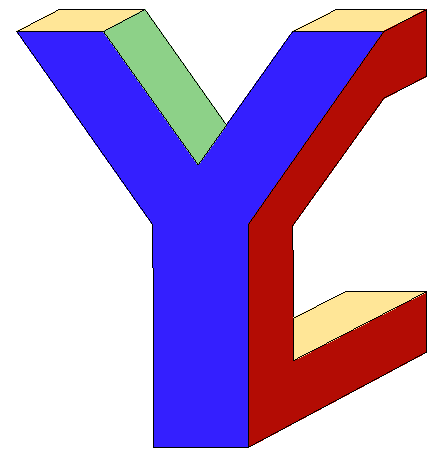
\includegraphics[height=1.5cm]{pictures/YC_logo.pdf}
    \end{center} 
  \end{tabular}
  \titlepage
\end{frame}
}

\begin{frame}[fragile]
  \transwipe[direction=90]
  \frametitle{Способы формализации}
  \begin{itemize}
    \item Грамматики Хомского
    \item Булевы граммтики   
    \item Языки и группы
    \item И ещё много разных подходов
  \end{itemize}
\end{frame}

\begin{frame}[fragile]
  \transwipe[direction=90]
  \frametitle{Булевы граммтики}
  \begin{itemize}
    \item Okhotin A. Conjunctive and Boolean grammars: the true general case of the context-free grammars //Computer Science Review. – 2013. – Т. 9. – С. 27-59.
    \item Okhotin A. Nine Open Problems on Conjunctive and Boolean Grammars //Bulletin of the EATCS. – 2007. – Т. 91. – С. 96-119.
    \item Kuznetsov S., Okhotin A. Conjunctive Categorial Grammars //Proceedings of the 15th Meeting on the Mathematics of Language. – 2017. – С. 140-151.
  \end{itemize}
\end{frame}


\begin{frame}[fragile]
  \transwipe[direction=90]
  \frametitle{Языки и группы}
  \begin{itemize}
    \item Anisimov A. V. Group languages //Cybernetics and Systems Analysis. – 1971. – Т. 7. – №. 4. – С. 594-601.
    \item Muller D. E., Schupp P. E. Groups, the theory of ends, and context-free languages //Journal of Computer and System Sciences. – 1983. – Т. 26. – №. 3. – С. 295-310.
    \item Salvati S. MIX is a 2-MCFL and the word problem in $\mathbb {Z}^ 2$ is solved by a third-order collapsible pushdown automaton //Journal of Computer and System Sciences. – 2015. – Т. 81. – №. 7. – С. 1252-1277.
    \item Nederhof M. J. A short proof that $ O_2 $ is an MCFL //arXiv preprint arXiv:1603.03610. – 2016.
    \item Ho M. C. et al. The word problem of $\mathbb {Z}^ n $ is a multiple context-free language //arXiv preprint arXiv:1702.02926. – 2017.
    \item Nesin R., Asli G. Descriptions of Groups using Formal Language Theory : дис. – Department of Computer Science, 2016.
  \end{itemize}
\end{frame}

\begin{frame}[fragile]
  \transwipe[direction=90]
  \frametitle{Другие подходы}
  \begin{itemize}
    \item Comon H. et al. Tree automata techniques and applications. Available on: h ttp //tata. gforge. inria. fr. release 12th October. – 2007.
    \item Rayward-Smith V. J. Hypergrammars: an extension of macrogrammars //Journal of Computer and System Sciences. – 1977. – Т. 14. – №. 1. – С. 130-149.
    \item Fischer M. J. Grammars with macro-like productions //Switching and Automata Theory, 1968., IEEE Conference Record of 9th Annual Symposium on. – IEEE, 1968. – С. 131-142.
    \item Schabes Y. Mathematical and computational aspects of lexicalized grammars. – 1990.
    \item Joshi A. K., Schabes Y. Tree-adjoining grammars //Handbook of formal languages. – 1997. – Т. 3. – С. 69-124.
  \end{itemize}
\end{frame}


\begin{frame}[fragile]
\transwipe[direction=90]
\frametitle{Пересечение языков/грамматик}
  \begin{itemize}
    \item Динамически формируемый код
    \item Графовые базы данных   
    \item Статический анализ кода
    \item Верификация
    \item Поиск в сжатом тексте
    \item ...
  \end{itemize}
\end{frame}

\begin{frame}[fragile]
\transwipe[direction=90]
\frametitle{Пересечение языков/грамматик 1}
  \begin{itemize}
    \item Verbitskaia E., Grigorev S., Avdyukhin D. Relaxed parsing of regular approximations of string-embedded languages //International Andrei Ershov Memorial Conference on Perspectives of System Informatics. – Springer International Publishing, 2015. – С. 291-302.
    \item Azimov R., Grigorev S. Graph Parsing by Matrix Multiplication //arXiv preprint arXiv:1707.01007. – 2017.
    \item Hellings J. Querying for Paths in Graphs using Context-Free Path Queries //arXiv preprint arXiv:1502.02242. – 2015.
    \item Bastani O., Anand S., Aiken A. Specification inference using context-free language reachability //ACM SIGPLAN Notices. – ACM, 2015. – Т. 50. – №. 1. – С. 553-566.
  \end{itemize}
\end{frame}

\begin{frame}[fragile]
\transwipe[direction=90]
\frametitle{Пересечение языков/грамматик 2}
  \begin{itemize}
    \item Nederhof M. J., Satta G. Parsing non-recursive context-free grammars //Proceedings of the 40th Annual Meeting on Association for Computational Linguistics. – Association for Computational Linguistics, 2002. – С. 112-119.
    \item Nederhof M. J., Satta G. The language intersection problem for non-recursive context-free grammars //Information and Computation. – 2004. – Т. 192. – №. 2. – С. 172-184.
    \item Zhang Q., Su Z. Context-sensitive data-dependence analysis via linear conjunctive language reachability //Proceedings of the 44th ACM SIGPLAN Symposium on Principles of Programming Languages. – ACM, 2017. – С. 344-358.
  \end{itemize}
\end{frame}


\begin{frame}[fragile]
\transwipe[direction=90]
\frametitle{Вывод грамматик}
  \begin{itemize}
    \item Clark A. Canonical context-free grammars and strong learning: two approaches //The 14th Meeting on the Mathematics of Language. – 2015. – С. 99.
    \item Clark A. Computational Learning of Syntax //Annual Review of Linguistics. – 2017. – Т. 3. – С. 107-123.
    \item Burghardt J. E-Generalization Using Grammars //arXiv preprint arXiv:1403.8118. – 2014.
    \item Clark A., Yoshinaka R. Distributional learning of context-free and multiple context-free grammars //Topics in Grammatical Inference. – Springer Berlin Heidelberg, 2016. – С. 143-172.
  \end{itemize}
\end{frame}
      
\begin{frame}[fragile]
\transwipe[direction=90]
\frametitle{Что ещё?}
\begin{itemize}
\item Fulop S. A., Kephart D. Topology of Language Classes //The 14th Meeting on the Mathematics of Language. – 2015. – С. 26.
\item Cai L., Malmberg R. L., Wu Y. Stochastic modeling of RNA pseudoknotted structures: a grammatical approach //Bioinformatics. – 2003. – Т. 19. – №. suppl\_1. – С. i66-i73.
\item Zier-Vogel R., Domaratzki M. RNA pseudoknot prediction through stochastic conjunctive grammars //Computability in Europe 2013. Informal Proceedings. – 2013. – С. 80-89.
\end{itemize}
\end{frame}

\end{document}
